%*******************************************************************************
%*********************************** First Chapter *****************************
%*******************************************************************************

\chapter{Introduction}
\label{chap:introduction}

Here is an example for referencing figure \ref{EnergySources}. Example of citing \cite{BP2019} and \cite{Chen2016}.
%%%%%%%%%%%%%% Figure: Energy sources
\begin{figure}[h]
	\centering
	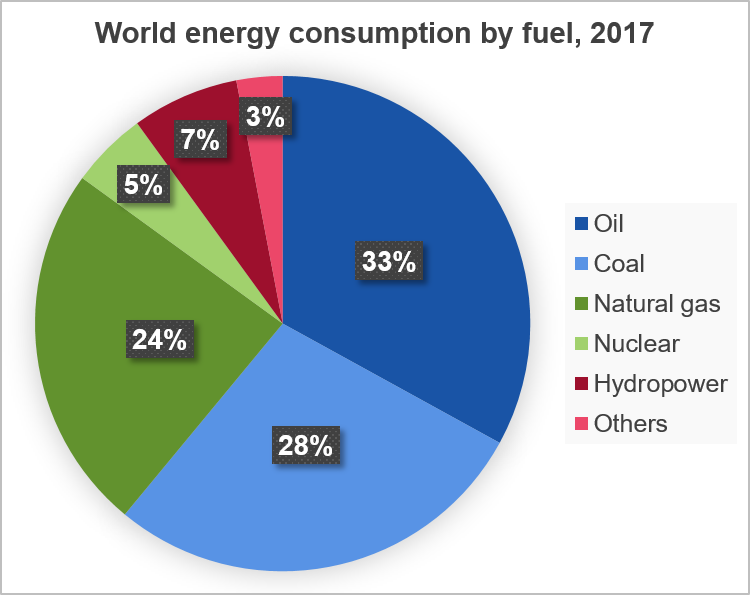
\includegraphics[scale=0.6]{Figs/Ch1_EnergySources.png}
	\caption{The world's energy consumption by fuel in 2017. }
	\label{EnergySources}
\end{figure}

%%%%%%%%%%%%%%%%%%%%%%%%%%%%%%%%%%%%%%%%
\section{Section}
Example of a table
%%%%%%%%%%%%%%%%%%%%%%%%%%%%%%%% Table: Tokamaks
\begin{table}[t!]
	\centering
	\caption{List of experimental tokamaks worldwide. Note: ITER is currently under construction and the first plasma is predicted for 2025-2028.}
	\begin{tabular}{ccccc}
		\hline
		\textbf{Name} & \textbf{Location} & \textbf{B-field} & \textbf{Major/minor radius}  \\
		\hline
		JET     & England      & 4.0 T & 3.0 m / 1.3 m \\
		ITER    & France       & 5.3 T & 6.2 m / 2.0 m \\
		AUG		& Germany      & 3.1 T & 1.7 m / 0.7 m \\
		WEST	& France	   & 3.7 T & 2.5 m / 0.5 m \\
		TCV     & Switzerland  & 1.5 T & 0.9 m / 0.3 m \\
		DIII-D  & USA          & 2.2 T & 1.7 m / 0.7 m \\
		TFTR 	& USA          & 6.0 T & 2.5 m / 0.9 m \\
		JT-60   & Japan        & 4.0 T & 3.4 m / 1.0 m \\
		K-STAR  & South Korea  & 3.5 T & 1.8 m / 0.5 m \\
		EAST    & China        & 3.5 T & 1.9 m / 0.5 m \\
		\hline
	\end{tabular}
	\label{TokamakTable}
\end{table}